\section{Experiments}
\label{sec:experiments}

We evaluate CJE on a large-scale benchmark. We initially expected doubly robust methods to dominate by combining logged data with fresh draws. Instead, we found two surprises: (i) OPE fails catastrophically even after weight stabilization boosts ESS above 90\%, and (ii) DR provides no advantage over Direct under low overlap, effectively reducing to the outcome model alone. These findings motivated the CLE bound and its TTC/AB diagnostics, which explain why high ESS is insufficient.

Our experiments address three questions:
\begin{enumerate}[leftmargin=*,itemsep=2pt,topsep=2pt]
\item Does calibration work? Reward calibration should reduce RMSE, improve ranking accuracy, and with calibration-aware inference restore valid CI coverage.
\item Why does OPE fail despite high ESS? We expected IPS to work after stabilization; CLE predicts failure when TTC is low.
\item Why doesn't DR dominate? Under low overlap, DR's IPS component contributes noise rather than information.
\end{enumerate}

\subsection{Experimental design}
\label{ssec:exp-setup}

\paragraph{Data.}
We started with 5,000 prompts from Chatbot Arena \citep{Zheng2023LLMasJudge}, a crowdsourced platform where users chat with anonymous LLMs. Prompts were randomly selected from first-turn English conversations; after filtering for teacher-forcing reliability, $n{=}4{,}961$ samples remain with complete data for all policies (see Limitations, \cref{sec:limitations}).

\paragraph{Policies.}
Five LLM configurations, each generating responses to all prompts:
\begin{itemize}[leftmargin=*,nosep]
\item \texttt{base}: Llama 3.3 70B with standard system prompt (logging policy $\pi_0$)
\item \texttt{clone}: Same model and prompt as base, different seed (TF reliability test)
\item \texttt{premium}: Llama 3.1 405B (model size effect)
\item \texttt{parallel\_universe\_prompt}: Llama 3.3 70B with modified system prompt (prompt engineering test)
\item \texttt{unhelpful}: Deliberately low-quality, confusing responses (adversarial stress test)
\end{itemize}
Total: ${\sim}25$k responses (${\sim}$5k prompts $\times$ 5 policies; $n{=}4{,}961$ after filtering).

\paragraph{Oracle and judge.}
\textbf{Oracle $Y$:} \texttt{gpt-5-2025-08-07} \citep{OpenAI2025GPT5} quality scores (0--100, normalized to $[0,1]$) collected for every response.
\textbf{Judge $S$:} \texttt{gpt-4.1-nano-2025-04-14} scores on all responses (temperature 0); approximately $16\times$ cheaper than oracle.\footnote{Pricing as of November 2025 via OpenAI API.}
\emph{Note:} The oracle model operates at temperature 1.0 (temperature 0 was not available for this model at experiment time), introducing stochasticity in oracle labels; we did not repeat-score responses, so coverage results may be conservative.
All estimators except \texttt{naive-direct} calibrate judge scores using reward calibration. Base variants use monotone-only calibration ($Z{=}S$); \texttt{+cov} variants use two-stage calibration with response length as a covariate ($Z{=}g(S,\text{length})$).
For DR methods, rewards $R=\hat f_{\mathrm{all}}(Z)$ use the full calibrator while the outcome model $\hat q=\hat f^{(-k)}(Z)$ uses cross-fitted (leave-one-fold-out) predictions; the difference $R-\hat q$ captures residual information for the IPS correction.

\paragraph{Experimental grid.}
We cross 13 estimators $\times$ 5 oracle fractions (5\%, 10\%, 25\%, 50\%, 100\%) $\times$ 5 sample sizes (500, 1k, 2k, 3k, 5k) $\times$ 50 random seeds = 16,250 total runs (1,250 per estimator). Reported metrics are means across seeds within each (oracle fraction, sample size) cell.

\paragraph{Metrics.}
\emph{Ranking:} Pairwise accuracy ($\text{PairAcc} = \binom{P}{2}^{-1}\sum_{j<k}\mathbf{1}\{(\hat V_j - \hat V_k)(V^\star_j - V^\star_k) > 0\}$, the fraction of correctly ordered policy pairs), Top-1 accuracy, Kendall's $\tau$.
\emph{Magnitude:} RMSE$^d$ (oracle-noise-debiased): $\mathrm{RMSE}^d = \sqrt{\max(0,\, \mathrm{MSE} - \widehat{\Var}(\bar Y))}$, where $\widehat{\Var}(\bar Y)$ is the variance of the oracle mean estimate (conservatively bounded by $0.25/n$ per policy). This isolates estimator error from irreducible oracle sampling noise.
\emph{Uncertainty:} Coverage (95\% CI capture rate).
\emph{Note:} Accuracy and uncertainty metrics exclude the \texttt{unhelpful} policy (which intentionally violates transportability); ranking metrics include all five policies to test whether estimators correctly identify the adversarial policy as worst.

\subsection{Results}
\label{ssec:exp-results}

\begin{table}[H]
\centering
\caption{Accuracy \& Uncertainty Metrics}
\label{tab:accuracy}
\setlength{\tabcolsep}{4pt} % tighten columns a bit
\resizebox{\linewidth}{!}{%
\begin{tabular}{lrrrrrrrr}
\toprule
Estimator & $\mathrm{RMSE}^{\mathrm{d}}$ $\downarrow$ & IS (interval score) $\downarrow$ & Coverage \\% $\to 95$ & SE GM $\downarrow$ & Pairwise \% $\uparrow$ & Top-1 \% $\uparrow$ & $\tau$ $\uparrow$ & Runtime (s) $\downarrow$ \\
\midrule
naive-direct & 0.0828 & 2.9580 & 0.0 & \textbf{0.0039} & 90.9 & 79.6 & 0.817 & 0.4 \\
direct & \textbf{0.0223} & \textbf{0.0542} & 85.0 & \underline{0.0068} & 91.8 & 84.1 & 0.837 & 0.7 \\
direct+cov & 0.0256 & \underline{0.0568} & 86.1 & 0.0074 & \textbf{94.4} & \textbf{89.5} & \textbf{0.888} & 1.6 \\
SNIPS & 0.1596 & 0.7379 & 98.3 & 0.1815 & 38.3 & 8.7 & -0.235 & \textbf{0.3} \\
SNIPS+cov & 0.1842 & 0.7544 & 97.8 & 0.1842 & 37.4 & 6.4 & -0.252 & \underline{0.3} \\
calibrated-ips & 0.0246 & 0.5727 & 99.1 & 0.0963 & 47.1 & 19.0 & -0.059 & 0.3 \\
calibrated-ips+cov & 0.0262 & 0.6084 & 99.2 & 0.1027 & 46.5 & 20.5 & -0.070 & 0.4 \\
dr-cpo & 0.0459 & 0.2203 & 99.2 & 0.0371 & 78.3 & 46.3 & 0.566 & 3.1 \\
dr-cpo+cov & 0.0570 & 0.2657 & 99.4 & 0.0449 & 79.1 & 50.1 & 0.581 & 9.6 \\
calibrated-dr-cpo & 0.0224 & 0.1357 & 99.5 & 0.0230 & 90.9 & 81.0 & 0.818 & 3.2 \\
calibrated-dr-cpo+cov & 0.0260 & 0.1398 & 99.3 & 0.0236 & \underline{94.1} & \underline{87.7} & \underline{0.882} & 9.7 \\
stacked-dr & \underline{0.0224} & 0.0788 & \textbf{95.6} & 0.0125 & 91.9 & 83.1 & 0.838 & 8.9 \\
stacked-dr+cov & 0.0281 & 0.0806 & \underline{96.1} & 0.0128 & 92.1 & 84.8 & 0.842 & 38.2 \\
\bottomrule
\end{tabular}
}
\footnotesize{
$\downarrow$: lower is better, $\uparrow$: higher is better, $\to 95$: target is 95\%. 
\textbf{Bold}: best (closest to target for Coverage \%), \underline{underlined}: second-best. 
Metrics averaged across all regimes.
}
\end{table}

\paragraph{Q1: Does calibration work?}
Yes, for both accuracy and inference. \Cref{tab:accuracy} shows calibration improves accuracy across method families.
For Direct: uncalibrated \texttt{naive-direct} achieves 90.9\% pairwise vs.\ calibrated \texttt{direct+cov} at 94.4\%.
For DR: raw-weight \texttt{dr} achieves 78.3\% pairwise ($\tau{=}0.57$) vs.\ weight-stabilized \texttt{calibrated-dr} at 90.9\% ($\tau{=}0.82$), a 12.6 percentage point gain (both use reward calibration; the gain is from weight stabilization).
For inference: uncalibrated CIs (\texttt{naive-direct}) achieve 0\% coverage: nominal 95\% CIs capture the true value in 0/50 seeds, a failure mode independently replicated by \citet{Chen2026EfficientLLMJudge}, who observe 0\% coverage for naive estimation under judge bias.
Bootstrap inference with bias-corrected estimation ($\hat\theta_{\mathrm{aug}}$) restores coverage: Direct achieves ${\sim}$95\% across oracle fractions (\cref{tab:uq-comparison}), as does stacked-DR.
The calibration uncertainty share of total variance ranges from 0\% (100\% oracle) to over 50\% (5\% oracle), explaining why ignoring calibration uncertainty produces catastrophically narrow CIs (\cref{fig:oua-decomposition}).

\begin{figure}[t]
  \centering
  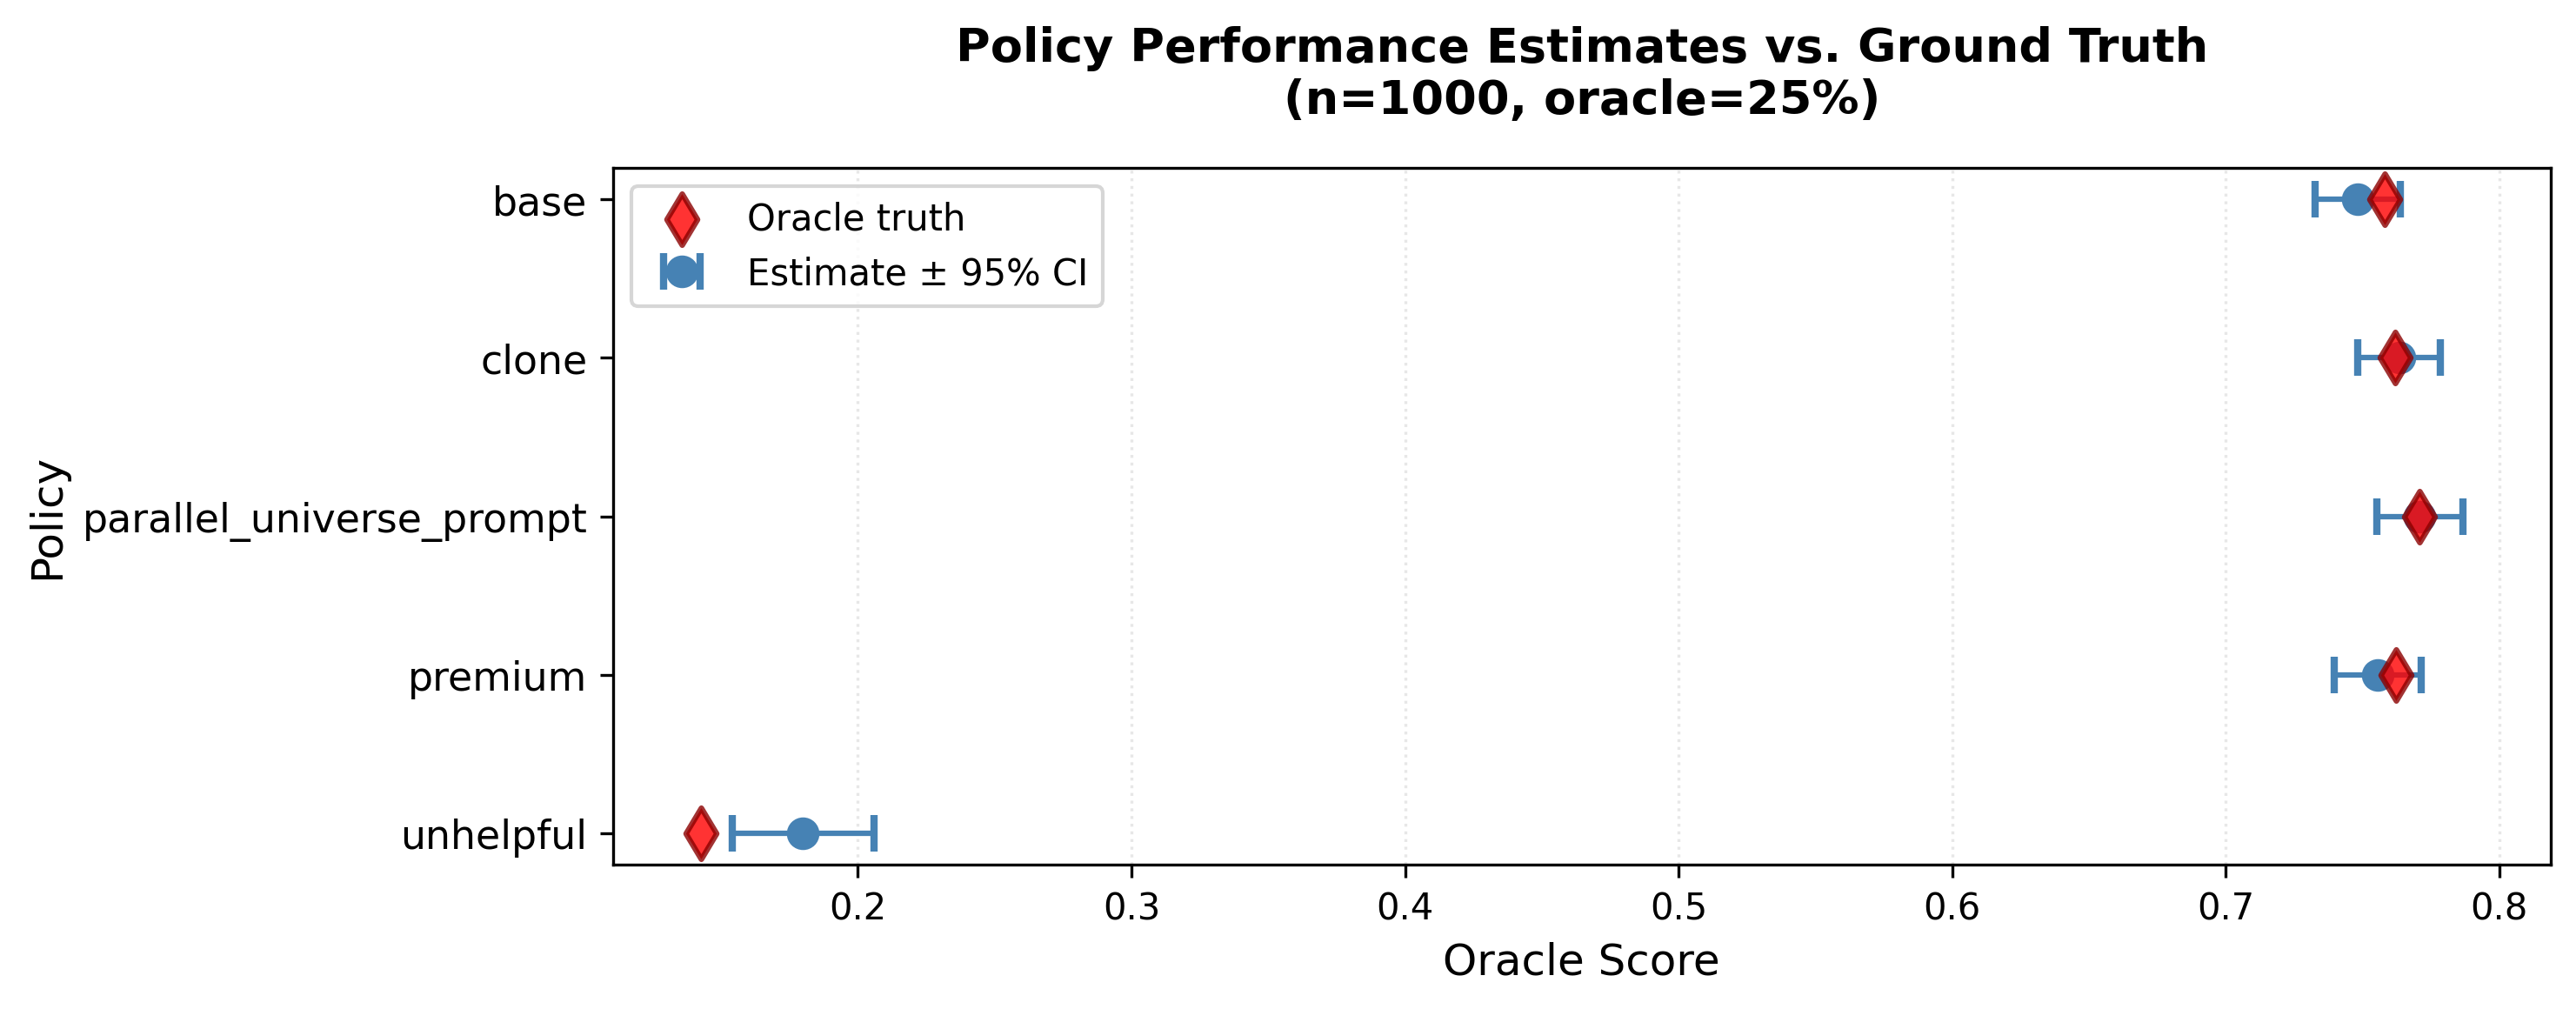
\includegraphics[width=\columnwidth]{figs/forest_plot_n1000_oracle25.png}
  \caption{\textbf{CJE output: policy value estimates at $n{=}1000$, 25\% oracle.} Red diamonds show oracle ground truth; blue circles show CJE estimates with 95\% CIs. CIs capture the true value for policies satisfying transportability; \texttt{unhelpful} (which violates transportability) shows slight miscoverage, a failure mode flagged by the transportability test (\cref{fig:transportability-test}).}
  \label{fig:forest-plot}
\end{figure}

\paragraph{Q2: Why does OPE fail despite high ESS?}
This was our main surprise. Despite weight stabilization boosting ESS from $<1\%$ to $>80\%$ for target policies, calibrated IPS ranking performance remains near-random: 47\% pairwise accuracy vs.\ 50\% chance baseline.
We expected weight stabilization to be sufficient; it was not.

OPE faces two compounding challenges in this setting.
\emph{First}, teacher-forcing logprobs are empirically unreliable: even for the clone policy (identical to logger), raw ESS is 26\% rather than the expected ${\sim}$100\% (\cref{tab:weight-diagnostics}), suggesting propensity estimates are corrupted by tokenization mismatches, API nondeterminism, or distribution shift between sampling and scoring.
\emph{Second}, even with stabilized weights, coverage-limited efficiency sets a hard precision floor: TTC ranges from 0.19 to 0.49 for non-clone policies, all below the 0.7 threshold, indicating the logger rarely visits target-typical regions. The resulting CLE factors (24--61$\times$) inflate standard errors beyond what any estimator can overcome.

\paragraph{Q3: Why doesn't DR dominate?}
We expected DR to outperform Direct by combining logged data with fresh draws. Instead, \texttt{direct+cov} slightly outperforms \texttt{calibrated-dr+cov} (94.4\% vs.\ 94.1\%).
The explanation: under low overlap, DR's IPS component contributes noise rather than information.
DR estimators are consistent if \emph{either} the propensity model \emph{or} the outcome model is correct.
Given IPS's failure, DR effectively relies \emph{entirely} on the outcome model $\hat{q}(Z)$, not the propensities.
This is exactly the regime CLE identifies: TTC is low, so logged data contributes little. DR $\approx$ Direct $+$ extra variance from unstable weights.
\emph{Implication:} When teacher forcing is unreliable, prefer Direct over DR; it achieves the same accuracy without requiring logprobs.

\begin{table}[t]
\centering
\caption{\textbf{Ablation: marginal contribution of CJE components.} Metrics averaged over 5 sample sizes $\times$ 5 oracle fractions $\times$ 50 seeds. CI coverage = \% of 95\% CIs containing truth (using bootstrap + $\hat\theta_{\mathrm{aug}}$ for Direct).}
\label{tab:ablation}
\small
\begin{tabular}{@{}lccr@{}}
\toprule
\textbf{Configuration} & \textbf{RMSE$^{\mathrm{d}}$} & \textbf{Coverage} & \textbf{$\Delta$RMSE$^{\mathrm{d}}$} \\
\midrule
\multicolumn{4}{l}{\textit{Effect of Reward Calibration}} \\
~~Direct, no calibration & 0.083 & 0\% & --- \\
~~Direct + reward calibration & 0.023 & 95\% & \textbf{--72\%} \\
\midrule
\multicolumn{4}{l}{\textit{Effect of Weight Stabilization}} \\
~~SNIPS (raw weights) & 0.160 & 98\% & --- \\
~~Calibrated-IPS (+ stabilization) & 0.025 & 99\% & \textbf{--84\%} \\
\midrule
\multicolumn{4}{l}{\textit{Combined Effect on DR}} \\
~~Calibrated DR, raw weights & 0.046 & 99\% & --- \\
~~Calibrated DR + stabilization & 0.023 & 100\% & --50\% \\
~~Calibrated DR + stabilization + cov & 0.026 & 99\% & --43\% \\
\midrule
\multicolumn{4}{l}{\textit{Recommended Configuration}} \\
~~\textbf{Direct + reward calibration + cov} & \textbf{0.026} & 95\% & \textbf{--69\%} \\
\bottomrule
\end{tabular}
\vspace{1mm}

\footnotesize{
\textbf{Key findings:} Reward calibration reduces RMSE by 72\% and restores coverage (0\%→95\% with bootstrap).
Weight stabilization reduces IPS RMSE by 84\%. Both contribute additively.
}
\end{table}


\begin{table}[t]
\centering
\caption{Coverage by UQ Method (target: 95\%). Bootstrap with calibrator refit achieves near-nominal coverage; cluster-robust and jackknife-only methods undercover.}
\label{tab:uq-comparison}
\small
\setlength{\tabcolsep}{4pt}
\begin{tabular}{lcccc}
\toprule
& \multicolumn{2}{c}{Analytic} & \multicolumn{2}{c}{Bootstrap} \\
\cmidrule(lr){2-3} \cmidrule(lr){4-5}
Regime & Cluster-Robust & Cal-Aware Jackknife & $B{=}500$ & $B{=}2000$ \\
\midrule
$n{=}250$, 5\% oracle & \textcolor{red}{21} & \textcolor{red}{85} & 94 & 93 \\
$n{=}250$, 25\% oracle & \textcolor{red}{43} & \textcolor{red}{86} & 95 & 97 \\
$n{=}500$, 5\% oracle & \textcolor{red}{28} & \textcolor{red}{89} & 96 & 97 \\
$n{=}500$, 25\% oracle & \textcolor{red}{40} & \textcolor{red}{84} & 98 & 99 \\
$n{=}1000$, 5\% oracle & \textcolor{red}{21} & \textcolor{red}{75} & 95 & 95 \\
$n{=}1000$, 25\% oracle & \textcolor{red}{35} & \textcolor{red}{83} & 95 & 95 \\
$n{=}2500$, 5\% oracle & \textcolor{red}{15} & \textcolor{red}{70} & 97 & 97 \\
$n{=}2500$, 25\% oracle & \textcolor{red}{52} & \textcolor{red}{85} & 98 & 99 \\
\bottomrule
\end{tabular}

\vspace{1mm}
\footnotesize{\textcolor{red}{Red}: $< 90\%$ (undercoverage). Bootstrap with $\hat\theta_{\mathrm{aug}}$ recommended.}
\end{table}


\paragraph{Component ablation.}
\Cref{tab:ablation} isolates the marginal contribution of each CJE component.
Reward calibration reduces RMSE by 72\% and is necessary to avoid catastrophic undercoverage: without it, 0\% of CIs contain the true value; with bootstrap inference, coverage improves to ${\sim}$95\%.
Weight stabilization reduces IPS RMSE by 84\% while maintaining coverage, validating the $S$-monotone projection approach.
\Cref{tab:uq-comparison} compares UQ methods for Direct mode: naive cluster-robust SEs achieve only 15--52\% coverage; calibration-aware jackknife improves to 70--89\%; bootstrap with $\hat\theta_{\mathrm{aug}}$ (AIPW-style residual augmentation) achieves ${\sim}$95\% by correcting both variance and bias from calibration uncertainty.

\begin{table}[t]
\centering
\caption{Weight Diagnostics: Weight Stabilization. Raw SNIPS weights have catastrophic ESS ($<1\%$) and heavy tails ($\alpha < 2$); weight stabilization recovers ESS $>80\%$ with light tails.}
\label{tab:weight-diagnostics}
\small
\setlength{\tabcolsep}{5pt}
\begin{tabular}{lcccccc}
\toprule
& \multicolumn{2}{c}{ESS (\%)}  & \multicolumn{2}{c}{Tail $\alpha$} & & \\
\cmidrule(lr){2-3} \cmidrule(lr){4-5}
Policy & SNIPS & Stab. & SNIPS & Stab. & TTC & CLE \\
\midrule
Clone & 26.2 & 99.0 & 1.08 & $>$10 & 79.6\% & 1.9$\times$ \\
Parallel Univ. & 0.6 & 95.4 & 0.56 & $>$10 & 49.4\% & 60.5$\times$ \\
Premium & 0.7 & 82.1 & 0.32 & $>$10 & 19.0\% & 23.8$\times$ \\
Unhelpful & 0.4 & 84.6 & 0.13 & $>$10 & 25.6\% & 37.6$\times$ \\
\bottomrule
\end{tabular}

\vspace{1mm}
\footnotesize{TTC = Target-Typicality Coverage; CLE = coverage-limited efficiency factor. Tail $\alpha < 2$ indicates infinite variance.}
\end{table}


\paragraph{Weight diagnostics.}
\Cref{tab:weight-diagnostics} quantifies the effect of weight stabilization and CLE diagnostics.
The mean-one isotonic projection reduces dispersion, yielding large ESS uplifts (e.g., from 0.6\% to 95\% for Parallel Universe), and tail relief (Hill $\alpha > 2$).
Yet ranking performance does not improve.
Note that even the clone policy---identical to logger---has raw ESS of only 26\%, far below the theoretical 100\%, reflecting teacher-forcing brittleness (see Limitations, \cref{sec:limitations}).
For non-clone policies, TTC ranges from 19--49\% with CLE factors of 24--61$\times$, indicating the logger rarely visits target-typical regions. Together, TF unreliability and CLE explain why high stabilized ESS does not translate to accurate ranking: propensity estimates are corrupted, and even perfect propensities would face a hard precision floor.

\begin{figure}[t]
  \centering
  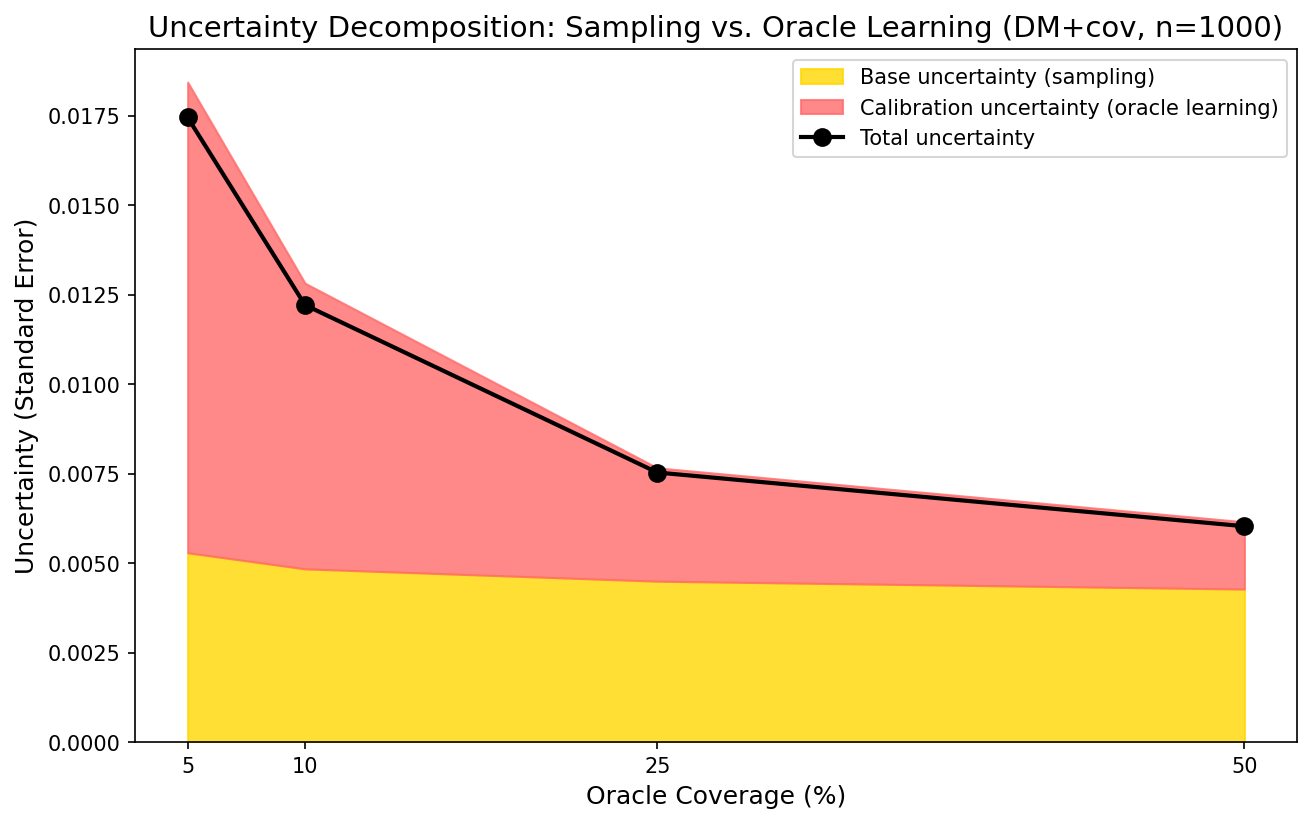
\includegraphics[width=\columnwidth]{figs/oua_vs_base_variance.png}
  \caption{\textbf{Uncertainty decomposition at $n{=}1000$ for \texttt{direct+cov}.}
  Yellow: base sampling uncertainty (constant ${\sim}$0.005). Orange: calibration uncertainty (dominates at low oracle fractions, contributing ${\sim}$90\% of total variance at 5\% oracle; shrinks to ${\sim}$30\% at 100\% because the estimator still fits a calibrator).}
  \label{fig:oua-decomposition}
\end{figure}

\begin{figure}[t]
  \centering
  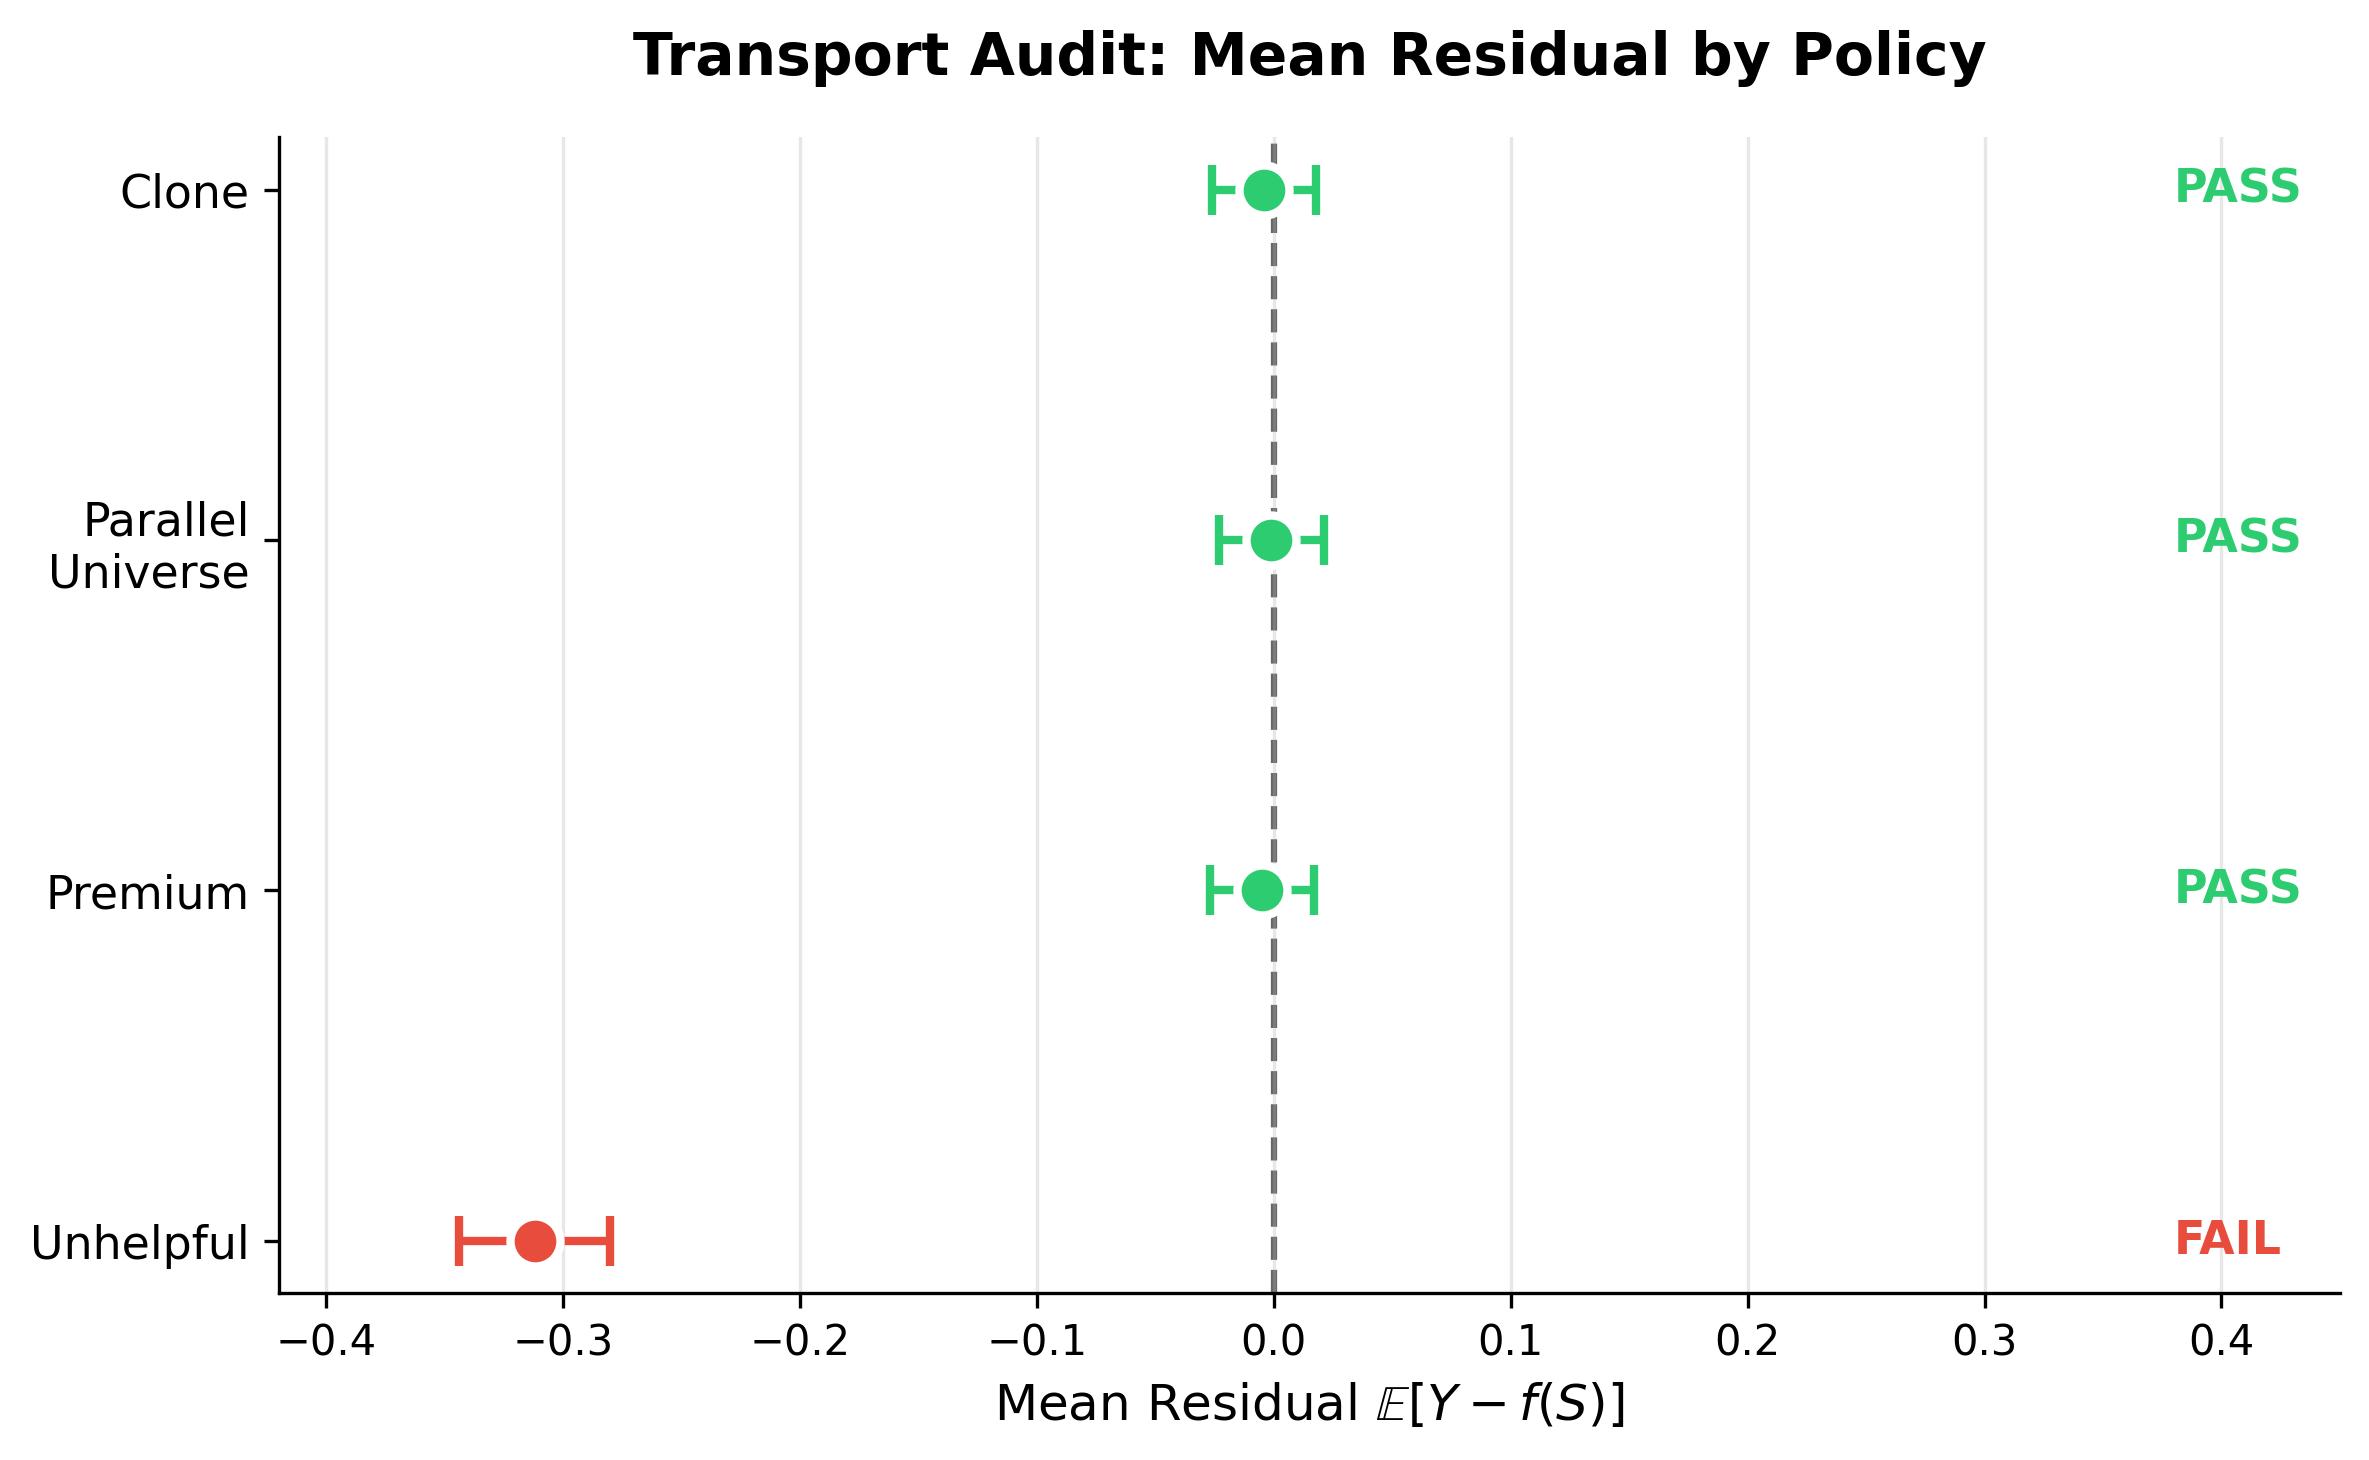
\includegraphics[width=\columnwidth]{figs/transportability_bar_chart.png}
  \caption{\textbf{Policy-wise mean transport test at 25\% oracle fraction.}
  Testing $H_{0,\pi'}: \E_{\pi'}[Y - f(S, X)] = 0$ per policy (Bonferroni-corrected $\alpha{=}0.0125$).
  Clone, Parallel Universe, and Premium pass (residuals centered at zero).
  Unhelpful fails (mean residual $= -0.31$): the surrogate overestimates oracle scores for adversarial responses by $+0.31$ in absolute level.}
  \label{fig:transportability-test}
\end{figure}

\paragraph{Calibration transportability.}
\Cref{fig:transportability-test} applies the policy-wise mean transport test (\cref{prop:mean-transport}) to validate whether the base-trained calibration can be reused across target policies.
We test $H_{0,\pi'}: \E_{\pi'}[Y - f(S,X)] = 0$ for each policy with Bonferroni correction ($\alpha{=}0.0125$).
Clone, Parallel Universe, and Premium all pass: their residual distributions are centered at zero, implying that Direct + calibrated surrogate remains mean-unbiased for these policies.
Unhelpful fails (mean residual $-0.31$, $p < 0.001$). By \cref{prop:mean-transport}, this implies $V^{\mathrm{oracle}}_{\pi'} - V^{\mathrm{sur}}_{\pi'} \approx -0.31$: the surrogate systematically \emph{overestimates} oracle quality for adversarial responses.
This flags a failure of mean transportability: absolute value estimates for this policy are biased, triggering the \textsc{REFUSE-LEVEL} gate (App.~\ref{app:diag-transport}).
Because Unhelpful's bias ($-0.31$) does not invert its rank relative to other policies (corrected value ${\approx}0.48$ remains well below ${\sim}0.75$), rankings remain valid; only absolute levels are refused.
\emph{Practical implication:} This test decides whether a single calibration can be safely reused across policies; if a policy fails, either recalibrate with policy-specific oracle data or fall back to oracle-only evaluation for that cell.
\emph{Remark (transport correction).} When transport fails, the estimated mean residual $\hat\Delta$ from the audit slice can serve as an intercept correction: $\hat V_{\mathrm{corr}} = \hat V_{\mathrm{sur}} + \hat\Delta$. However, we recommend refusing level claims by default, as the correction only fixes the mean and policy-specific recalibration is preferable when feasible.

\paragraph{Judge-policy confound.}
When a model judges its own outputs, transport can fail due to self-preference bias. On MBPP code generation (\cref{app:mbpp}), GPT-4o-mini judging its own outputs showed a significant mean residual ($-0.065$, $p{=}0.006$). Never judge a model with itself without auditing transport; this failure mode cannot be fixed by calibration alone.

\subsection{Comparison to Misclassification Correction}
\label{ssec:binary}

A natural alternative to continuous calibration is misclassification correction~\citep{RoganGladen1978}, recently adapted for LLM judges by~\citet{Lee2025LLMJudgeReporting}. Both approaches are calibration-based; they differ in what signal they use (continuous vs.\ thresholded) and in how uncertainty propagates. Lee et al.\ assume \emph{confusion-matrix stability}---that $\Pr(\hat Z \mid Z)$ is constant across distributions---analogous to our transport condition.

\paragraph{Setup.} This comparison uses a separate experiment from the main benchmark, designed for an apples-to-apples evaluation with Lee et al.'s binary setting.
We test on 9,999 Arena preference pairs (50.5\% A-wins), the most favorable domain for binary methods: mean Youden's $J = 0.41$ across policies, compared to $J = 0.05$ on code correctness where binary estimation is ill-conditioned. Both methods are evaluated on the same 3 target policies (verbose, terse, contrarian) with identical oracle budgets, test splits, seeds, and judge model (gpt-4o-mini). Confidence intervals follow~\citet{Lee2025LLMJudgeReporting} Eq.~6 with Agresti-Coull adjustment.

\begin{table}[t]
\centering
\small
\caption{\textbf{Misclassification correction vs.\ continuous calibration on Arena preferences} (mean Youden's $J \approx 0.41$). Both methods achieve near-nominal 95\% CI coverage, but CJE produces $9\times$ narrower confidence intervals while achieving 93\% lower RMSE even when Rogan-Gladen uses the optimal threshold.}
\label{tab:binary-comparison}
\begin{tabular}{lccc}
\toprule
Method & RMSE & 95\% CI Coverage & CI Half-Width \\
\midrule
CJE (direct) & $\mathbf{0.004}$ & 96.4\% & $\mathbf{0.015}$ \\
Rogan-Gladen ($\tau{=}0.5$) & $0.063$ & 95.6\% & 0.135 \\
Rogan-Gladen ($\tau{=}0.6$, best) & $0.061$ & 98.9\% & 0.136 \\
\bottomrule
\end{tabular}
\vspace{1mm}
\par\noindent{\footnotesize \emph{Setup:} 9,999 Arena preference pairs (50.5\% A-wins); 3 target policies (verbose, terse, contrarian); identical oracle budgets per cell. CIs follow~\citet{Lee2025LLMJudgeReporting} Eq.~6. Threshold $\tau$ binarizes the continuous judge score; $\tau{=}0.5$ is the natural argmax, $\tau{=}0.6$ is optimal from a sweep over $\{0.3, 0.4, 0.5, 0.6, 0.7\}$.}
\end{table}


\paragraph{Results.} \Cref{tab:binary-comparison} shows both methods achieve near-nominal coverage. However, even with the optimal threshold ($\tau{=}0.6$), CJE achieves 93\% lower RMSE (0.004 vs.\ 0.061) and $9\times$ narrower confidence intervals (half-width 0.015 vs.\ 0.136).

\paragraph{Why the gap?} Two factors explain the efficiency difference:
(1)~\emph{Ill-conditioning}: the Rogan-Gladen estimator $\hat\theta = (\hat p + \widehat{Sp} - 1)/J$ has standard error scaling like $1/J$; at $J \approx 0.44$, small errors in $(\hat p, \widehat{Se}, \widehat{Sp})$ amplify into large errors in $\hat\theta$.
(2)~\emph{Information loss}: binary thresholding discards the continuous probability signal that CJE exploits.
We swept thresholds $\tau \in \{0.3, 0.4, 0.5, 0.6, 0.7\}$ to rule out suboptimal binarization; the best ($\tau{=}0.6$) is shown in the table.

\paragraph{Implication.} Even when misclassification correction is numerically well-conditioned ($J$ well above zero), continuous calibration remains substantially more sample-efficient. Both approaches require transportability diagnostics: Lee et al.'s method relies on confusion-matrix stability; CJE relies on score transport. The key difference is that CJE makes diagnostics \emph{actionable}---we gate the calibrated estimator on transport passing, preventing calibration from damaging estimates when the assumption fails. CJE also generalizes beyond preferences: on MBPP code generation with unit-test ground truth, calibration reduces RMSE by 32--84\% for transport-valid policies at 10\%+ oracle fraction (\cref{app:mbpp}).

\paragraph{Distribution shift robustness.}
\citet{Lee2025LLMJudgeReporting} emphasize that their estimator is robust to shifts in $\Pr(Z)$ between calibration and test sets (their Section~7), since confusion-matrix parameters $\Pr(\hat Z \mid Z)$ do not depend on $\Pr(Z)$.
We tested this claim by varying the calibration-set class balance while holding the test set at its natural rate ($\Pr(Z{=}1) \approx 0.51$).
Results confirm their prediction: Rogan-Gladen bias remains near zero across all shifts (mean $|\mathrm{bias}| < 0.007$), while CJE bias scales linearly with the calibration--test mismatch ($-0.14$ at $\Pr(Z{=}1)_{\mathrm{calib}}{=}0.30$, $+0.14$ at $0.70$).
This is a genuine advantage of confusion-matrix methods: when practitioners cannot control the calibration distribution, misclassification correction provides robustness that continuous calibration lacks.
However, when calibration and test distributions match---the typical experimental design---CJE's efficiency advantage dominates (RMSE $0.009$ vs.\ $0.032$ at no shift).

\paragraph{Sample size planning.}
\Cref{fig:mde-contours} shows MDE contours for the Direct Method: the smallest true policy difference detectable at 80\% power, 5\% two-sided significance.
Key observation: for a fixed label budget $m = n \times \text{oracle fraction}$, larger $n$ with lower oracle fraction outperforms smaller $n$ with higher oracle fraction, suggesting \emph{spread labels across more samples} as a practical rule.
\emph{Practical guidance:} For new domains, oversample the first batch (e.g., $n{=}2{,}000$ with 25\% oracle fraction) to generate a domain-specific MDE plot, then use it to select the minimal viable $(n, \text{oracle fraction})$ for future experiments.

\begin{figure}[t]
  \centering
  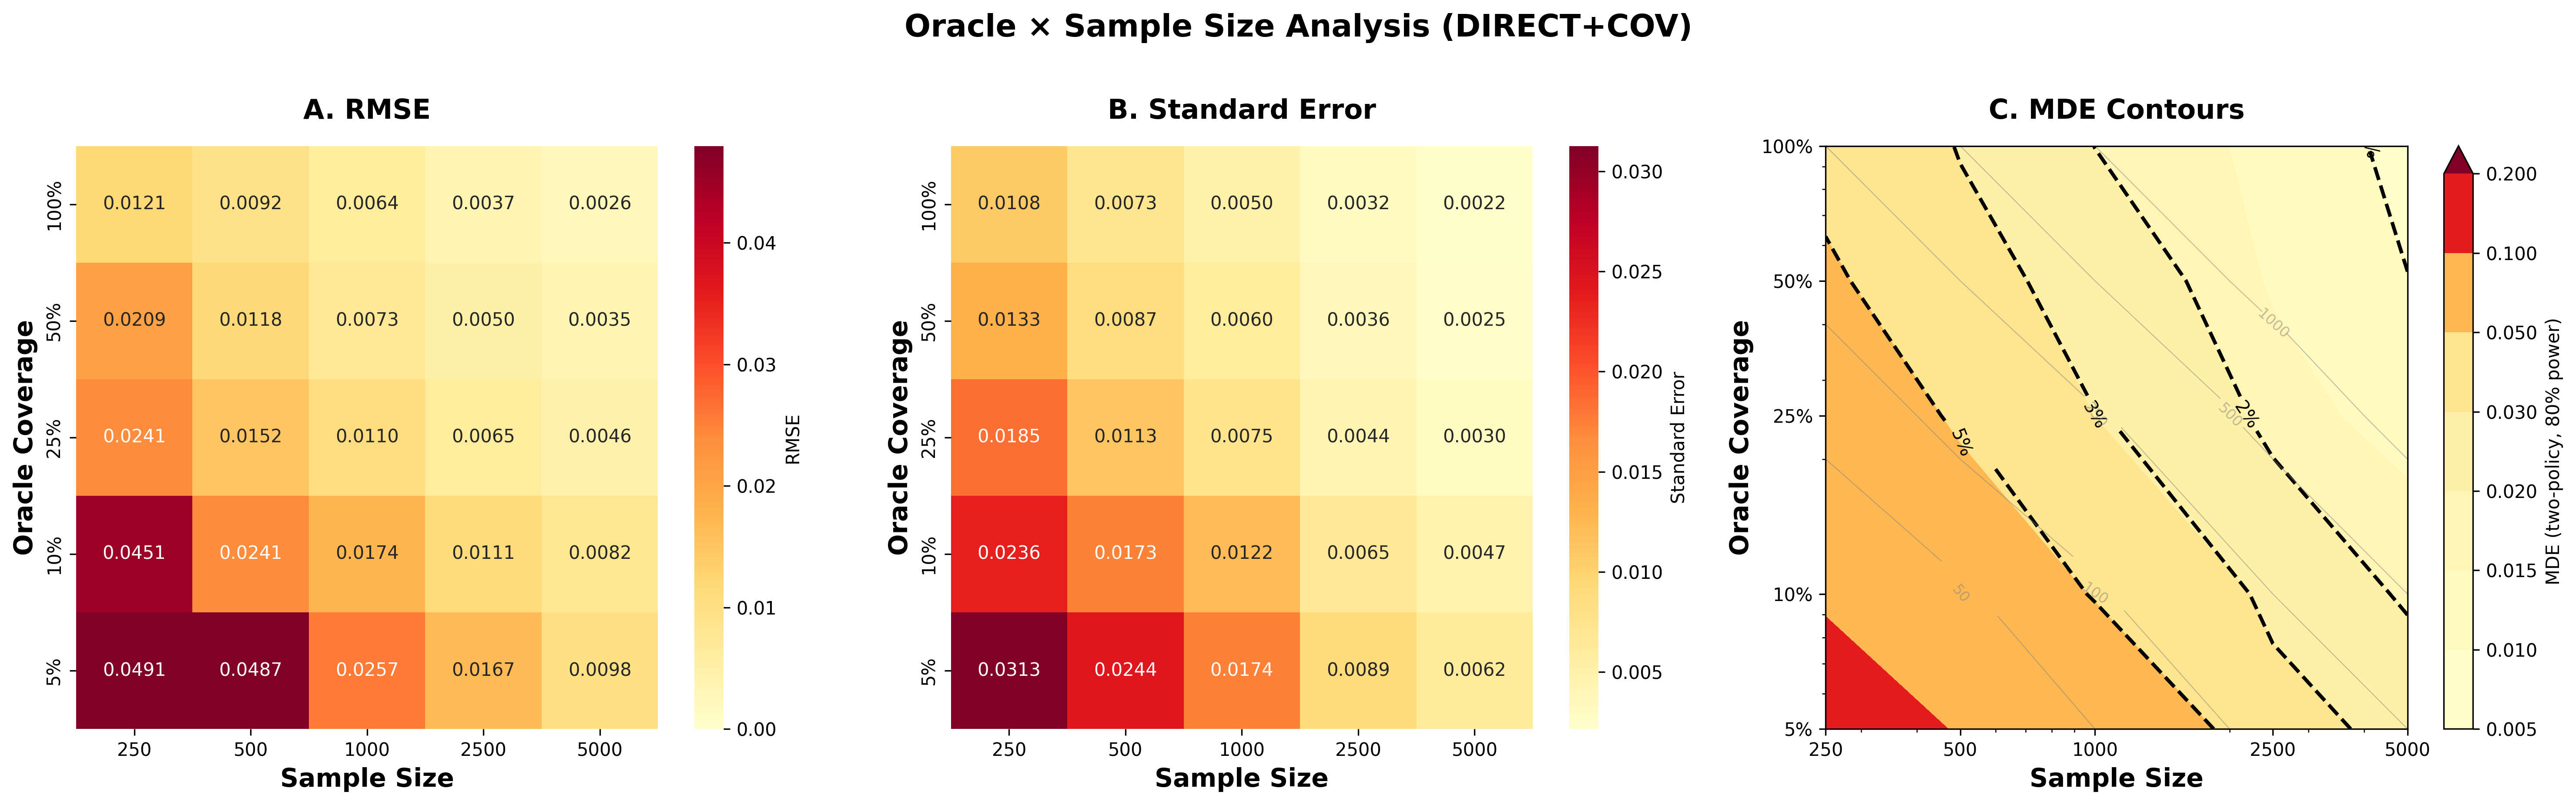
\includegraphics[width=\columnwidth]{figs/mde_direct_cov.png}
  \caption{\textbf{Sample size planning for \texttt{direct+cov}.}
  (A) RMSE by sample size and oracle fraction.
  (B) Standard errors including calibration uncertainty.
  (C) MDE contours showing the smallest effect detectable at 80\% power.
  Dashed lines show common detection thresholds; cells with MDE $< 0.02$ enable detecting 2-point quality differences.
  For a fixed label budget, spread labels across more samples (larger $n$, lower oracle \%) rather than concentrating labels on fewer samples.}
  \label{fig:mde-contours}
\end{figure}

\paragraph{Cost analysis.}
\Cref{tab:cost-analysis} quantifies the cost-accuracy tradeoff.
CJE with 5\% oracle calibration achieves 99\% pairwise ranking accuracy at $n{=}5{,}000$ (98.7\% averaged over 50 seeds) at \textbf{14$\times$ lower total cost} than pure oracle labeling (for all 5 policies).
Oracle labels cost approximately $16\times$ more than judge scores, so total cost scales primarily with oracle fraction.
At 5\% oracle fraction, this yields an 8.8$\times$ cost reduction for a single policy.
With amortization across 5 policies, this becomes 14$\times$ (see below), enabling scaling to production workloads where pure oracle labeling is prohibitive.
Amortization improves further: calibrating once on a shared oracle slice enables evaluating multiple policies at marginal judge-only cost, approaching the 16$\times$ cost ratio as $P$ grows.
\emph{Sensitivity:} At smaller $n$ or higher oracle fractions, the cost advantage shrinks; at 25\% oracle fraction the reduction is 3.5$\times$. Ranking accuracy depends on policy gaps and transport validity: the 94\% average across all configurations (\cref{tab:accuracy}) is more representative than the 99\% peak.

\begin{table}[h]
\centering
\small
\caption{\textbf{Cost-accuracy tradeoff} for $n{=}5{,}000$ prompts $\times$ 5 policies (rounded for cost arithmetic; experiments use $n{=}4{,}961$ after filtering). CJE achieves near-oracle accuracy at 14$\times$ lower cost.\textsuperscript{$\dagger$}}
\label{tab:cost-analysis}
\begin{tabular}{lrrrr}
\toprule
Method & Oracle Cost & Judge Cost & Total & Pairwise \% \\
\midrule
Pure oracle (100\%) & \$55.00 & -- & \$55.00 & 100\% \\
CJE (5\% oracle) & \$0.55 & \$3.50 & \textbf{\$4.05} & 99\% \\
\bottomrule
\end{tabular}
\vspace{1mm}
\par\noindent{\footnotesize \textsuperscript{$\dagger$}Costs exclude one-time calibration audits (transportability tests, residual diagnostics). These add ${\sim}$10--20\% overhead initially but amortize across subsequent evaluations on the same domain.}
\end{table}

\begin{table}[h]
\centering
\small
\caption{\textbf{Estimator Selection Guide.} Requirements and recommended use cases for each estimator family.}
\label{tab:estimator-guide}
\begin{tabular}{@{}lcccp{4cm}@{}}
\toprule
\textbf{Estimator} & \textbf{Fresh} & \textbf{Logprobs} & \textbf{Overlap} & \textbf{When to Use} \\
\midrule
Direct & \checkmark & -- & -- & \textbf{Default} for LLM eval \\
IPS/SNIPS & -- & \checkmark & Required & Small policy changes only \\
Calibrated IPS & -- & \checkmark & Required & + weight stabilization \\
DR & \checkmark & \checkmark & Helpful & Logs + fresh draws available \\
Stacked-DR & \checkmark & \checkmark & Helpful & Production ensemble \\
\bottomrule
\end{tabular}
\end{table}

\subsection{Practical takeaways}
\label{ssec:takeaways}

\begin{enumerate}[leftmargin=*,itemsep=2pt,topsep=2pt]
\item Default to Direct + two-stage calibration. For open-ended generation under nontrivial policy shifts, logs-only OPE faces two compounding issues: TF brittleness and coverage sparsity. Direct requires no overlap assumption and achieves the best ranking accuracy in our benchmark (\cref{tab:estimator-guide}).
\item Audit transport for high-stakes decisions. When reporting absolute values or making deployment decisions, run the mean transport test on a small oracle slice per target policy (or time window). Pass $\to$ reuse calibration; fail $\to$ recalibrate with policy-specific data or refuse level claims for that cell. For exploratory analysis or ranking-only comparisons, the audit can be deferred.
\item Gate on TTC before relying on logged data. If TTC $< 0.70$, CLE implies a precision floor that weight stabilization cannot overcome; in our benchmark, only near-clone policies pass this threshold. For constrained settings (short outputs, near-clone shifts), OPE may remain viable; verify with diagnostics before trusting logged-data estimates.
\item Always use bootstrap inference with $\hat\theta_{\mathrm{aug}}$. Standard CIs severely under-cover (15--52\%); calibration-aware jackknife improves but still falls short (70--89\%); bootstrap with bias correction achieves near-nominal coverage (${\sim}$95\%).
\item Use calibration uncertainty share to guide resource allocation. The fraction $\widehat{\mathrm{Var}}_{\mathrm{cal}} / \widehat{\mathrm{Var}}_{\mathrm{total}}$ identifies bottlenecks: if calibration uncertainty share $> 50\%$, collect more oracle labels; if calibration uncertainty share $< 20\%$, collect more evaluation prompts (\cref{fig:oua-decomposition}).
\item Covariates matter. Response length as a calibration covariate (not a reweighting covariate) improves ranking across all methods.
\item Optimize the budget ratio. How many oracle labels do you need? The optimal ratio of labels ($m$) to scores ($n$) follows a square-root law based on costs and variances (\cref{app:budget}). Check the calibration uncertainty share $\omega$ to equalize marginal utility: if $\frac{\omega}{1-\omega} > \frac{\mathrm{Spend}_{\mathrm{oracle}}}{\mathrm{Spend}_{\mathrm{surrogate}}}$, the experiment is under-investing in oracle labels.
\end{enumerate}
